
%%%%%%%%%%%%%%%%% Introduction to the Assignment %%%

In this Assignment, \textit{\textbf{Problem 4 - Pulse modulation techniques and observations of the atmosphere}}, ...


%%%%%%%%%%%%%%%%% TASK 1 %%%
\section{Pulse coding techniques}

\subsection{Normalized ambiguity diagram}

\subsection{Amplitude normalized auto-correlation function}

\subsection{Radar system properties}

\subsection{Detectability}

\subsection{Properties of the ambiguity function}

\subsection{Ambiguities in the diagram}

\subsection{Pulse amplitude and pulse width of two radar systems}

\subsection{Comparison of Barker coding and no coding}

\subsection{Comparison of Barker and complementary coding}

\subsection{Comparison of PRN and no coding}

\subsection{Comparison of LFM and no coding}


%%%%%%%%%%%%%%%%% TASK 2 %%%
\section{Reduction of effective height resolution}

\subsection{Signal-to-noise ratio as function of time}
Using the provided datasets, captured on 28th February 2006, the Signal-to-Noise ratio is plotted against altitude and local time. The associated MATLAB-Code can be found in Appendix \ref{apx:matlab}. The Code used is similar to the one used in \textit{Problem 2 - General Radar Theory} to plot SNR against altitude and time.

\begin{figure}
	\centering
	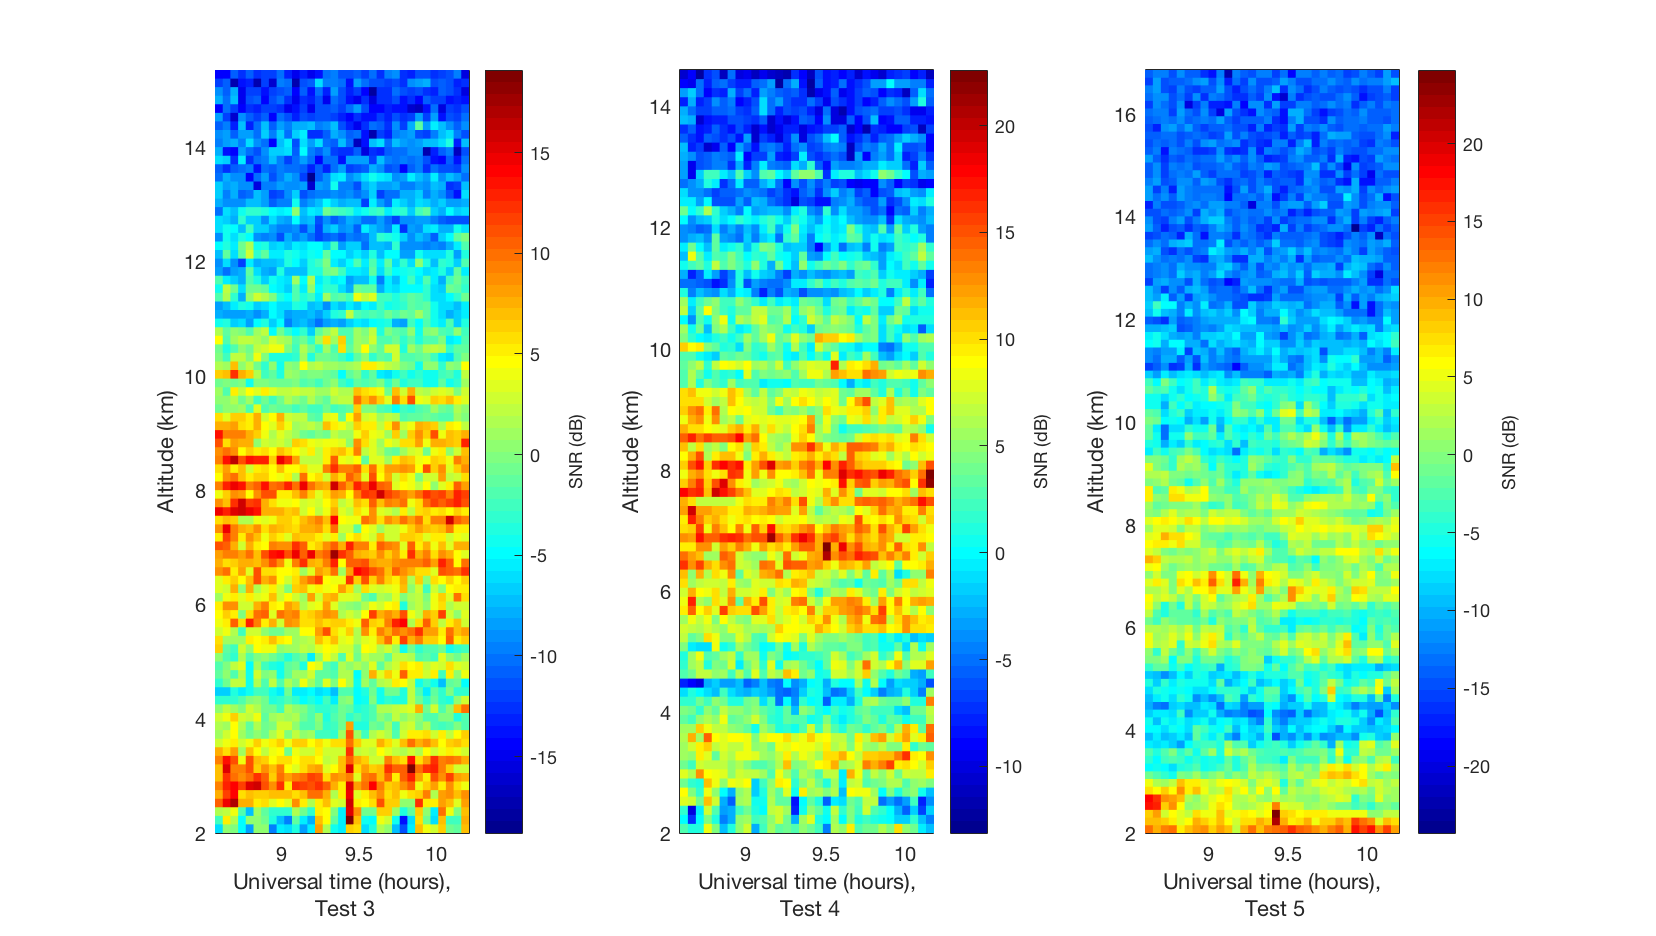
\includegraphics[width=0.9\textwidth]{images/task2_snr_plot}
	\caption{SNR against altitude and time for each dataset}
	\label{fig:snr}
\end{figure}

Each dataset for the three tests contains radar data with different coding techniques; test 3 has Barker coding, test 4 complementary coding and test 5 has uncoded data. \newline



\subsection{Scientific usability of obtained data plots}
As one can easily see in Fig. \ref{fig:snr}, test 4, the complementary coding has the highest SNR compared to the other two tests. Thus it seems that this dataset can give the most detailed view of the atmosphere, concerning.
Although one could argue, that the SNR is almost too high, since the region between 5 and 10 km is almost. \todo{what to write here?}
\subsection{Dynamical state of the atmosphere}









